\documentclass[runningheads]{llncs}
%
% LayerTree: constant-size exit and eviction from a shared Bitcoin UTXO.
% Build: latexmk -pdf main.tex   (or: make)
%
\usepackage[T1]{fontenc}
\usepackage[utf8]{inputenc}
\usepackage{microtype}
\usepackage{amsmath,amssymb}
\usepackage{booktabs}
\usepackage{multirow}
\usepackage{graphicx}
\usepackage{xcolor}
\usepackage{tikz}
\usetikzlibrary{positioning,arrows.meta,calc,fit,backgrounds,shapes.misc}
\usepackage{pgfplots}
\pgfplotsset{compat=1.18}
\usepackage[n,operators,sets,adversary,landau,probability,notions,logic,ff,mm,primitives,events,complexity,asymptotics,keys]{cryptocode}
\usepackage{listings}
\lstset{basicstyle=\ttfamily\scriptsize, columns=fullflexible, keepspaces=true,
  breaklines=true, breakatwhitespace=true, frame=none, xleftmargin=1em,
  aboveskip=4pt, belowskip=4pt, extendedchars=true,
  literate={→}{{$\rightarrow$}}1 {∀}{{$\forall$}}1 {∃}{{$\exists$}}1
    {∧}{{$\wedge$}}1 {∨}{{$\vee$}}1 {≠}{{$\neq$}}1 {≤}{{$\le$}}1 {×}{{$\times$}}1
    {π}{{$\pi$}}1 {₁}{{$_1$}}1 {₂}{{$_2$}}1 {′}{{$'$}}1 {⟨}{{$\langle$}}1 {⟩}{{$\rangle$}}1
    {∈}{{$\in$}}1 {¬}{{$\neg$}}1 {ₙ}{{$_n$}}1}
\usepackage[hidelinks]{hyperref}
\usepackage{url}

\newcommand{\Hleaf}{\ensuremath{H_{\mathsf{leaf}}}}
\newcommand{\Hnode}{\ensuremath{H_{\mathsf{node}}}}
\newcommand{\Hstate}{\ensuremath{H_{\mathsf{state}}}}
\newcommand{\Hpos}{\ensuremath{H_{\mathsf{pos}}}}
\newcommand{\NUMS}{\ensuremath{\mathsf{NUMS}}}
\newcommand{\spk}{\ensuremath{\mathsf{spk}}}
\newcommand{\TreeSpk}{\ensuremath{\mathsf{TreeSPK}}}
\newcommand{\fold}{\ensuremath{\mathsf{fold}}}
\newcommand{\encs}{\ensuremath{\mathsf{enc}_{64}}}
\newcommand{\lesf}{\ensuremath{\mathsf{le}_{64}}}
\newcommand{\op}[1]{\texttt{OP\_#1}}
\newcommand{\tr}[1]{\textsf{#1}}
\newcommand{\vB}{\,\mathrm{vB}}
\newcommand{\WU}{\,\mathrm{WU}}
\newcommand{\sat}{\,\mathrm{sat}}
\newcommand{\Emp}{\ensuremath{E}}
\newcommand{\lean}[1]{{\small\textsf{#1}}}

\begin{document}

\title{LayerTree: Constant-Size Exit and Eviction\\ from a Shared Bitcoin UTXO}
\titlerunning{LayerTree}
\author{Olaoluwa Osuntokun}
\authorrunning{O. Osuntokun}
\institute{Lightning Labs\\ \email{laolu@lightning.engineering}}

\maketitle

\begin{abstract}
Constructions that let many users share one Bitcoin output pay for the
sharing at exit time: a user who leaves unilaterally publishes a chain of
$O(\log N)$ transactions, the interior of the sharing tree must exist as
pre-signed or template-committed transactions, and one unresponsive user
forces the whole tree on-chain when it expires. We present
\textsc{LayerTree}, in which a single output commits to an off-chain
Merkle-sum tree of $N$ balances and tapscript covenants enforce every
state transition. Any member exits, and the operator evicts any expired
member, in one transaction whose size is independent of $N$: 1{,}020
virtual bytes for a tree of 65{,}536 positions, about 2.5$\times$ less
than unrolling an Ark- or CTV-style tree of the same size. Membership
changes need no interactive signing round, the shared output never
expires, and whole cohorts are added or swept in one constant-shape
transaction (158 virtual bytes per evicted leaf).

The construction composes only opcodes already proposed for Bitcoin: the
restored script opcodes of tapleaf version \texttt{0xC2}, transaction
introspection, signature checks over stack messages and elliptic-curve
tweaks. We give three complete realisations for decreasing opcode sets and
show that \op{CAT} plus one point-tweak opcode suffice, by having the
script rebuild the BIP-341 signature message and check it with a
generator-key signature. We show how Lightning channels are hosted inside
leaves with prevout-independent commitments, so that a hub of $N$ channels
occupies one output. We prove conservation, proof soundness and
unconditional payability in the idealised hash model and mechanise the
proofs in Lean~4. A Python simulator, a Go implementation cross-checked
byte for byte against it, and 338 executable checks accompany the design.
\keywords{Bitcoin \and covenants \and Merkle-sum trees \and payment
channels \and layer two \and formal verification}
\end{abstract}

\section{Introduction}

Bitcoin's throughput is bounded by block space, and the settled answer is
to move activity off-chain while keeping the chain as the court of last
resort. Payment channels~\cite{lightning} do this for pairs; the open
problem is doing it for \emph{groups}: letting $N$ users share one
unspent transaction output (UTXO) without giving up the ability of each to
leave alone. Every deployed or proposed approach to this problem pays for
the sharing when it is dissolved. In channel factories~\cite{factories},
Ark~\cite{ark}, timeout trees~\cite{timeouttrees} and
covenant trees built on \op{CHECKTEMPLATEVERIFY}~\cite{bip119} or
\op{CHECKCONTRACTVERIFY}~\cite{bip443,matt}, the shared output is the root
of a tree of \emph{transactions}. A member who leaves unilaterally must
publish the path from the root to its leaf, $O(\log N)$ transactions each
paying a fee; the interior of the tree must exist in advance as pre-signed
transactions (requiring every member to sign, and to be online) or as
covenant templates; and when the tree expires, reclaiming the funds of a
single unresponsive member means publishing everything.

This paper takes a different route. The tree stays entirely off-chain and
is a tree of \emph{data}, not transactions: a binary Merkle-sum tree
whose leaves are balances and whose root is committed by one output. A
member exits by presenting its leaf and its sibling path to the output
itself. The spending script recomputes the root from the proof, checks it
against the commitment, recomputes the root with the leaf removed, and
requires the transaction to recreate the output under the new root with
exactly the leaf's amount paid out. The member needs nobody's signature,
the exit is one transaction, and its size grows with the depth of the
tree rather than with the number of transactions in a path. The same
covenant lets the operator evict a member whose lease has expired, graft
a pre-built subtree of new members in one step, and sweep an expired
cohort at a small fraction of the per-leaf cost.

What makes this possible is a set of script capabilities that have been
proposed for Bitcoin but are not yet consensus: the restoration of the
disabled string and arithmetic opcodes in a new tapleaf version
(``Great Script Restoration'', BIPs~440 and 441~\cite{bip440,bip441}),
transaction introspection (\op{TX}~\cite{optx}), signature verification
over stack data (\op{CHECKSIGFROMSTACK}~\cite{bip348}), and
elliptic-curve point arithmetic~\cite{ecops,bip449}. We deliberately
propose no opcode of our own. The design is an argument about what the
candidate set buys, and part of the contribution is a precise account of
how little of it is actually needed.

\paragraph{Contributions.}
\begin{enumerate}
\item \textbf{Construction} (\S\ref{sec:construction}). A shared output
  committing to a Merkle-sum tree through a data-tweaked taproot internal
  key, with transitions for unilateral exit, eviction, batched exit,
  subtree grafting, cooperative update, single-use vouchers and cohort
  sweeps. Two tree profiles are specified: a dense operator-assigned tree
  and a key-addressed sparse tree with compressed proofs.
\item \textbf{Realisation in three opcode tiers} (\S\ref{sec:scripts}).
  Every transition is implemented against the full candidate set, against
  a \texttt{0xC0}-only subset, and against the minimum we could find:
  \op{CAT} and one point-tweak opcode. The last tier replaces
  introspection by a constructive trick, rebuilding the BIP-341 signature
  message in script and checking a signature under the generator point.
\item \textbf{Channel leaves} (\S\ref{sec:channels}). Lightning channels
  hosted in leaves, with commitment signatures that bind to no prevout
  (an \texttt{ANYPREVOUT} emulation from \op{TX} and
  \op{CHECKSIGFROMSTACK}) and an update/settlement state machine, so a
  channel's funding output need not exist until a dispute. We identify
  three tree-layer rules that hosting shared-key leaves requires.
\item \textbf{Security analysis with mechanised proofs}
  (\S\ref{sec:security}). Conservation, proof soundness and payability
  are proved in the idealised hash model and checked in Lean~4. The
  proofs isolated two facts the informal argument had blurred: sums are
  conserved unconditionally, but exits are guaranteed only under grafted
  nodes that have preimages.
\item \textbf{Implementation and measurement} (\S\ref{sec:eval}). A
  tapscript simulator for the candidate opcodes, a Go implementation
  matched byte for byte against it, and measured costs: a unilateral exit
  of $1{,}020\vB$ at depth~16, a marginal batched exit of $665\vB$, cohort
  eviction at $158\vB$ per leaf, and fee tables from 1 to 250
  sat/vB.
\end{enumerate}
The specification, code and proofs are public~\cite{layertreerepo}.

\section{Background}\label{sec:background}

\paragraph{Taproot and tapscript.}
A pay-to-taproot output~\cite{bip341} commits to an internal public key
$P$ and a Merkle root $m$ of a \emph{taptree} of scripts; the output key
is $Q = P + H_{\mathsf{TapTweak}}(P \,\|\, m)\cdot G$. An output is spent
either by a Schnorr signature~\cite{bip340} under $Q$ or by revealing one
script together with its Merkle path (the \emph{control block}) and
satisfying it. Tapscript~\cite{bip342} is a stack language without loops;
every ``loop'' below is unrolled and its cost is linear in the number of
iterations. A leaf's version byte selects its semantics.

\paragraph{Candidate opcodes.}
BIP-441~\cite{bip441} defines tapleaf version \texttt{0xC2}, in which the
string opcodes disabled in 2010 (\op{CAT}, \op{SUBSTR}, \op{LEFT},
\op{RIGHT}, bitwise operations and shifts) are restored and arithmetic is
on unsigned numbers of arbitrary length, with BIP-440~\cite{bip440}
metering the runtime cost (``varops''). \op{TX}~\cite{optx} pushes
selected fields of the spending transaction (its inputs' amounts and
scripts, its outputs, lock time), optionally collated into one hash
preimage. \op{CHECKSIGFROMSTACK}~\cite{bip348} verifies a Schnorr
signature over an arbitrary stack element. \op{TWEAKADD}~\cite{bip449}
computes the x coordinate of $P + t\cdot G$; the EC-ops draft~\cite{ecops}
generalises this to point addition, scalar multiplication and negation.
All are proposals; we treat them as given and note where the design
depends on details that are still open.

\paragraph{Merkle-sum trees.}
A Merkle-sum tree~\cite{merkle,mssmt} stores at every node the hash of
its children together with the sum of the values below it, and hashes the
children's sums into the parent. An inclusion proof for a leaf therefore
proves not only membership but the leaf's contribution to the root sum,
and the root sum is a commitment to the total. Sparse Merkle
trees~\cite{smt} address positions by hash, so that non-membership is an
inclusion proof of an empty leaf.

\section{Model and Goals}\label{sec:model}

A \emph{tree} has one \emph{operator} and any number of \emph{members}.
Each member owns a \emph{leaf}: a balance together with three public keys
(an owner key that authorises the member's actions, an exit key to which
the balance is paid on exit, and an evictor key, normally the operator's,
that may remove the leaf after a lease height). The operator holds no
special key over the funds; it holds an \emph{operator key} that
authorises additions to the tree and co-signs cooperative changes. A
\emph{tree output} is the on-chain UTXO. Its amount equals the sum of all
leaf balances, and its script commits to the tree root.

We assume the Bitcoin consensus and mempool rules with the opcodes of
\S\ref{sec:background} active, collision-resistant tagged hashing
(SHA-256), the discrete-logarithm assumption on secp256k1, and
unforgeable Schnorr signatures. The adversary controls the operator, any
subset of members, and the order of transactions within the rules; it
may refuse to serve data. We want:

\begin{description}
\item[G1 Conservation.] No transition creates value: the tree output's
  amount is always the sum of the leaf balances committed by its root,
  and every payout is funded by a leaf that the transition removes.
\item[G2 Unilateral constant-size exit.] A member holding its leaf and
  sibling path can always construct an accepted exit paying its balance,
  in one transaction whose size is independent of $N$, with no signature
  from any other party.
\item[G3 Eviction.] After a leaf's lease height its evictor can remove it,
  paying the balance to the leaf's exit key, so that an unresponsive
  member cannot pin the tree.
\item[G4 Non-interactive membership.] Adding or removing members requires
  no signing round among existing members and no pre-signed transactions.
\item[G5 No expiry.] The shared output has no lifetime; leases are per
  leaf and renewable.
\end{description}
Liveness of \emph{joins} is not a goal: a malicious operator may refuse
to add members, and members may refuse to be added. Data availability is
a member's responsibility (\S\ref{sec:discussion}).

\section{Construction}\label{sec:construction}

\subsection{The Tree}\label{sec:tree}

Fix a depth $D$. A tree has $2^D$ positions, each empty or holding a leaf.
A leaf is a fixed 116-byte record:
\begin{multline*}
\lesf(\mathsf{amount}) \,\|\, \mathsf{exit\_key} \,\|\, \mathsf{owner\_key}
\,\|\, \mathsf{evictor\_key} \\
\,\|\, \mathsf{le}_{32}(\mathsf{evict\_after})
\,\|\, \mathsf{le}_{32}(\mathsf{nonce}) \,\|\, \mathsf{le}_{32}(\mathsf{seq}),
\end{multline*}
with keys as 32-byte x-only points, $\mathsf{evict\_after}$ a block
height, $\mathsf{nonce}$ a per-leaf identifier and $\mathsf{seq}$ a
counter advanced by vouchers (\S\ref{sec:claim}). A \emph{node} is a pair
$(h, s)$ of a 32-byte hash and an unsigned sum. A position holding leaf
$\ell$ has node $(\Hleaf(\ell), \ell.\mathsf{amount})$; an empty position
has node $\Emp_0 = (0^{32}, 0)$. The parent of $(h_L, s_L)$ and
$(h_R, s_R)$ is
\[
\bigl(\Hnode(h_L \,\|\, \encs(s_L) \,\|\, h_R \,\|\, \encs(s_R)),\; s_L + s_R\bigr),
\qquad \encs(s) = \lesf(s) \,\|\, \mathtt{0x01}.
\]
$\Hleaf$ and $\Hnode$ are BIP-340 tagged hashes with distinct tags. The
encoding $\encs(s)$ is chosen so that a script can produce it from a
computed sum with a single addition: under BIP-441 numerics the minimal
encoding of $s + 2^{64}$ is exactly $\lesf(s)\,\|\,\mathtt{01}$ for
$s < 2^{64}$ (Lemma~\ref{lem:enc}). We write $\Emp_h$ for the root of the
empty tree of height $h$; these constants are hard-coded in scripts.

The \emph{sibling path} of a position is the list of $D$ pairs
$(\mathsf{dir}_k, (h_k, s_k))$, one per level, giving the direction taken
and the sibling node not taken. $\fold(n, \pi)$ combines a node $n$ with a
path $\pi$ level by level, hashing $n$ with its sibling in the order the
direction bit gives and adding the sums, and returns the implied root.
The two facts that drive the design are that the honest path folds a
leaf's node to the root, and that folding a \emph{different} node up the
\emph{same} path yields the root of the tree with that position replaced
(\S\ref{sec:security}).

\paragraph{Profiles.}
In the \emph{dense} profile positions are assigned by the operator and a
path carries explicit direction bits; each level costs 88 bytes of script
and 41 bytes of witness. In the \emph{sparse} profile a leaf's position is
the low $D$ bits of $\Hpos(\mathsf{owner\_key} \,\|\, \mathsf{nonce})$,
direction bits are derived in script from the position hash, and empty
siblings are elided from the witness (a one-byte marker in place of a
node; the script substitutes $\Emp_k$). The sparse profile is the
Merkle-sum sparse Merkle tree of Taproot Assets~\cite{mssmt} truncated to
$D = 32$ or $64$ levels: it gives key-addressed positions, a
history-independent root and structural uniqueness of leaves, at about
twice the per-exit cost of the dense profile
(Table~\ref{tab:sizes}). A 256-level tree costs about twelve times as much
and buys nothing beyond the ability to use a raw key as a position.

\subsection{The Tree Output}\label{sec:output}

Let $r$ be the root hash and $S$ the root sum. The tree output is a
taproot output with internal key
\[
P = \NUMS + \Hstate(r)\cdot G,
\]
where $\NUMS$ is the BIP-341 nothing-up-my-sleeve point, so the key path is
unspendable and every spend goes through a script. Its taptree contains
one leaf per supported transition script; the taptree's Merkle root $m$
identifies the rule set and is constant for the tree's life. We write
$\TreeSpk(r, m)$ for the resulting scriptPubKey. A tree output for state
$(r, S)$ is an output with script $\TreeSpk(r, m)$ and amount $S$.

Every transition script receives $r$ and $m$ in its witness, recomputes
$\TreeSpk(r, m)$, and checks that it equals the scriptPubKey of the input
being spent, read with \op{TX}. This binds both the root the proofs are checked against and
the script set the successor output will carry. The scripts cannot
hard-code $m$ because $m$ depends on them; taking $m$ from the witness and
verifying it resolves the circularity, and binding it is security
critical: a spender who could substitute $m'$ would recreate the tree
under scripts of its choosing.

\begin{figure}[t]
\centering
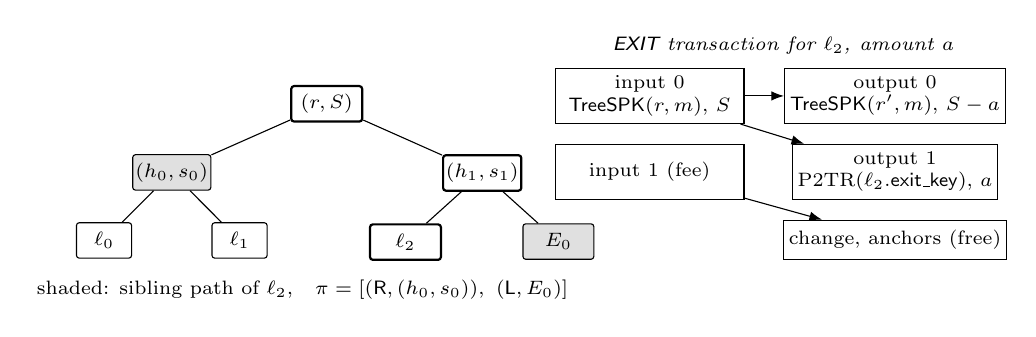
\begin{tikzpicture}[
  node distance=4mm and 2mm,
  every node/.style={font=\scriptsize},
  tn/.style={draw, rounded corners=1pt, minimum width=9mm, minimum height=4.5mm, inner sep=1pt},
  sib/.style={tn, fill=black!12},
  path/.style={tn, thick},
  leaf/.style={tn, minimum width=7mm},
  box/.style={draw, minimum height=7mm, align=center, inner sep=2pt},
  arr/.style={-{Latex[length=1.6mm]}, thin}
]
% tree (left)
\node[path] (root) {$(r,S)$};
\node[sib, below left=of root, xshift=-8mm] (n0) {$(h_0,s_0)$};
\node[path, below right=of root, xshift=8mm] (n1) {$(h_1,s_1)$};
\node[leaf, below left=of n0, xshift=2mm] (l00) {$\ell_0$};
\node[leaf, below right=of n0, xshift=-2mm] (l01) {$\ell_1$};
\node[path, below left=of n1, xshift=2mm] (l10) {$\ell_2$};
\node[sib, below right=of n1, xshift=-2mm] (l11) {$\Emp_0$};
\draw (root) -- (n0); \draw (root) -- (n1);
\draw (n0) -- (l00); \draw (n0) -- (l01);
\draw (n1) -- (l10); \draw (n1) -- (l11);
\node[below=1.5mm of l01, xshift=8mm, align=center] {shaded: sibling path of $\ell_2$,\quad $\pi = [(\mathsf{R}, (h_0,s_0)),\ (\mathsf{L}, \Emp_0)]$};
% transaction (right)
\begin{scope}[xshift=41mm, yshift=1mm]
\node[box, minimum width=24mm] (in0) {input 0\\ $\TreeSpk(r,m)$, $S$};
\node[box, minimum width=24mm, below=2.5mm of in0] (in1) {input 1 (fee)};
\node[box, minimum width=26mm, right=5mm of in0] (out0) {output 0\\ $\TreeSpk(r',m)$, $S-a$};
\node[box, minimum width=26mm, below=2.5mm of out0] (out1) {output 1\\ $\mathrm{P2TR}(\ell_2.\mathsf{exit\_key})$, $a$};
\node[box, minimum width=26mm, minimum height=5mm, below=2.5mm of out1] (out2) {change, anchors (free)};
\draw[arr] (in0) -- (out0);
\draw[arr] (in0) -- (out1);
\draw[arr] (in1) -- (out2);
\node[above=0.5mm of in0, xshift=17mm, font=\scriptsize\itshape] {\tr{EXIT} transaction for $\ell_2$, amount $a$};
\end{scope}
\end{tikzpicture}
\caption{A depth-2 tree and the exit of $\ell_2$. The output commits to $(r,S)$ through $\TreeSpk(r,m)$. The script checks $\fold((\Hleaf(\ell_2),a),\pi) = (r,S)$, computes $r' = \fold(\Emp_0,\pi)$, verifies a signature by $\ell_2.\mathsf{owner\_key}$, and constrains outputs 0 and 1; everything else in the transaction is free.}
\label{fig:exit}
\end{figure}

\subsection{Transitions}\label{sec:transitions}

Every transition spends the tree output as input~0 and recreates it as
output~0 with the new root and the new total; payouts, if any, occupy
outputs $1, \dots, K$; all other inputs and outputs are unconstrained, so
fees, change and anchors are free. The common core of every transition is
the \emph{step} of Figure~\ref{fig:step}: given a path $\pi$, an old node
and a new node, check that the old node folds to the committed root and
compute the root the new node folds to.

\begin{figure}[t]
\centering
\begin{pcvstack}[center]
\scalebox{0.9}{\procedure[linenumbering]{$\mathsf{Step}(\pi, n_{\mathrm{old}}, n_{\mathrm{new}}, (r, S))$}{
  (r_0, S_0) \gets \fold(n_{\mathrm{old}}, \pi) \pccomment{$D-h$ unrolled levels} \\
  \pcassert r_0 = r \wedge S_0 = S \pccomment{\tr{CHECK\_OLD}: $S$ is input 0's amount} \\
  (r', S') \gets \fold(n_{\mathrm{new}}, \pi) \pccomment{same siblings, same sums} \\
  \pcreturn (r', S')
}}
\pcvspace
\scalebox{0.9}{\procedure[linenumbering]{$\mathsf{Final}((r', S'), m)$}{
  \pcif (r', S') = \Emp_D \pcthen \pcreturn \pccomment{terminal: output 0 free} \\
  (a_0, \spk_0) \gets \op{TX}(\text{output } 0) \\
  \pcassert \spk_0 = \TreeSpk(r', m) \wedge a_0 = S'
}}
\end{pcvstack}
\caption{The Merkle-sum step shared by all transitions, and the output rule. A transition is a sequence of steps, each proving its old node against the root the previous step produced (\tr{CHECK\_PREV}), followed by \textsf{Final}. Authorisation and payout checks are specific to each transition.}
\label{fig:step}
\end{figure}

\paragraph{\tr{EXIT}.} Removes one leaf $\ell$: the old node is
$(\Hleaf(\ell), \ell.\mathsf{amount})$, the new node is $\Emp_0$.
Output~1 must pay to $\mathrm{P2TR}(\ell.\mathsf{exit\_key})$. The
witness carries a flag selecting one of two authorisations. An
\emph{owner exit} requires a signature over the transaction by
$\ell.\mathsf{owner\_key}$ and permits output~1's amount to be at most
$\ell.\mathsf{amount}$ (the difference is available as fee, and the owner
consented to it by signing). An \emph{eviction} requires a signature by
$\ell.\mathsf{evictor\_key}$, a lock time of at least
$\ell.\mathsf{evict\_after}$, and output~1's amount \emph{equal} to
$\ell.\mathsf{amount}$: an evictor may remove but never shortchange. The
signature must cover all outputs (\texttt{SIGHASH\_DEFAULT} or
\texttt{ALL}); otherwise a relayer could redirect the fee slack. An
\emph{exact-payout variant} \tr{EXIT}$^{=}$ requires equality for owner
exits too; it is a tree-creation parameter and matters for shared-key
leaves (\S\ref{sec:channels}).

\paragraph{\tr{JOIN}$_h$.} Grafts a subtree of height $h$ into an empty
aligned slot: the old node is the constant $\Emp_h$, the new node
$(h_{\mathrm{new}}, s_{\mathrm{new}})$ is supplied by the operator and
authorised by its signature, and output~0's amount rises by
$s_{\mathrm{new}}$, which other inputs must fund. With $h = 0$ this adds
one leaf; with $h = 8$ it adds up to 256 members for the same constant
script cost. The covenant does not verify the interior of the grafted
subtree, and cannot: prospective members verify their own paths inside it
before funding the join (\S\ref{sec:security}). \tr{JOINK}$_K$ sequences
$K$ single-leaf joins under one operator signature, which is the batching
primitive of the sparse profile, where positions are not
operator-assignable and grafting is unavailable.

\paragraph{\tr{UPDATE}.} Replaces one leaf by another at the same position
with signatures from both the owner and the operator; the output amount
moves by the difference. This is the splice, the lease renewal and the
ownership transfer. A variant \tr{UPDATE}$^{x}$ additionally requires a
signature by the \emph{old} leaf's exit key, for leaves whose exit key is
shared with a third party (\S\ref{sec:channels}).

\paragraph{\tr{CLAIM}.}\label{sec:claim} Executes a \emph{voucher}: an
off-chain, owner-signed instruction to carve a new leaf out of an existing
one. The voucher is a BIP-340 signature by the source leaf's owner over
$H_{\mathsf{voucher}}(m \,\|\, \ell_{\mathrm{src}} \,\|\, \ell_{\mathrm{claim}})$,
verified with \op{CHECKSIGFROMSTACK}. The transition is two steps: the
source leaf's amount is reduced by the claim amount and its $\mathsf{seq}$
advanced by one (or the position emptied if drained), then the claim leaf
is placed at an empty position. The total is unchanged. Replay is
impossible because the first step changes the source leaf, so the signed
message never again matches a leaf in the tree; the $\mathsf{seq}$ field
prevents a balance that later returns to an earlier value from
re-enabling an old voucher. Vouchers are the mechanism for
operator-to-member push payments without the operator's later
participation; they are optional.

\paragraph{Composition.} \tr{EXIT}$_K$ applies $K$ exits in one
transaction, each authorised independently, paying outputs $1..K$; the
$k$-th step proves its leaf against the root produced by step $k-1$.
\tr{EVICT\_SUBTREE}$_h$ is a \emph{shape-specialised multiproof}: it
takes one sibling path to an aligned subtree of height $h$ and the
$2^h$ leaves below it (or empty markers), recomputes the subtree's root
from them in post-order, checks each leaf's evictor key equals the
operator key and its lease has expired, pays each leaf to its exit key at
the next unused output, and replaces the subtree by $\Emp_h$. It hashes
the subtree's internal nodes once instead of once per leaf, which is what
makes cohort eviction cheap (\S\ref{sec:eval}). A generic
flag-driven multiproof was measured and rejected: it does not reduce
script size, since script has no loops to share.

\paragraph{Terminal transitions.} If the new root is $\Emp_D$ the tree is
empty and output~0 is unconstrained, so a tree can be dissolved without
leaving a zero-value output.

\section{Script Realisation and Opcode Tiers}\label{sec:scripts}

Every transition of \S\ref{sec:transitions} is realised three times,
against three opcode sets (Table~\ref{tab:tiers}), so that the design's
dependence on each candidate opcode is measured rather than asserted. The
tree format is identical in every tier; only the scripts differ.

\begin{table}[t]
\centering\small
\caption{The three opcode tiers. Sizes are bytes of script / witness data for \tr{EXIT}$_1$ in the dense profile at $D=16$.}
\label{tab:tiers}
\setlength{\tabcolsep}{3.5pt}\scriptsize
\begin{tabular}{@{}lccc@{}}
\toprule
 & \textbf{FULL} & \textbf{MID} & \textbf{MIN} \\
\midrule
Tapleaf version & \texttt{0xC2} & \texttt{0xC0} & \texttt{0xC0} \\
Numerics & unsigned, any length & 4-byte \texttt{CScriptNum} & 4-byte \texttt{CScriptNum} \\
Beyond BIP-342 & \op{CAT}, splice, bit ops; \op{TX}; & \op{CAT}; \op{TX}; & \op{CAT}; \op{TWEAKADD} \\
 & \op{CSFS}; EC point ops & \op{CSFS}; \op{TWEAKADD} & \\
Introspection & \op{TX} & \op{TX} & constructive (\S\ref{sec:min}) \\
Leaf on the stack & one 116-byte element & seven fields, re-joined & seven fields, re-joined \\
Sum limit per tree & none & $2^{31}$ sat & $2^{31}$ sat \\
Vouchers (\tr{CLAIM}) & yes & yes & no \\
Channel leaves & yes & yes & no \\
Transaction shape & free & free & fixed (2 inputs) \\
\tr{EXIT}$_1$, $D=16$ & 2{,}101 / 902 & 3{,}299 / 978 & 3{,}572 / 1{,}175 \\
\bottomrule
\end{tabular}
\end{table}

\subsection{The FULL Tier}
With \texttt{0xC2} the leaf is a single 116-byte stack element whose
fields are read with \op{SUBSTR}; sums are added with arbitrary-length
arithmetic and padded with $\langle 2^{64}\rangle\ \op{ADD}$
(Lemma~\ref{lem:enc}); each \tr{LEVEL} of the fold is 88 bytes:
concatenate the two 41-byte encodings in the order the direction bit
gives, tagged-hash, add the sums. $\TreeSpk$ is recomputed with the EC
opcodes: $\Hstate(r)$ is multiplied onto $G$, added to $\NUMS$, tweaked
by the taptree hash, and its x coordinate wrapped in a P2TR script. The
whole \tr{EXIT}$_1$ prologue, including both introspections and the key
recomputation, is under 700 bytes; depth costs 88 bytes per level.

\subsection{The MID Tier}
Tapleaf \texttt{0xC0} keeps BIP-342 semantics: no splice opcodes and
4-byte signed numbers. Two gadgets bridge the gap. Fields arrive as
separate witness elements, each checked with \op{SIZE} and re-joined with
\op{CAT} before hashing. A computed sum is widened to a fixed 8 bytes by a
witness-supplied zero pad $z$ and filler $w$ with
$z\,\|\,w = \mathtt{00000000}$ and $|x| + |z| = 4$, so that $x\,\|\,z$ is the
little-endian 4-byte form of $x$ (\textsf{PADZ}). \texttt{MINIMALDATA}
policy forbids using raw little-endian fields as numbers, so lock times
and positions arrive as minimal numbers plus a pad. The cap of
$2^{31}$ satoshis per tree (about 21.47 BTC) is the price of 4-byte
arithmetic. Everything in the design survives, at about 1.6$\times$ the
script size. The tier assumes \op{TX} is available in \texttt{0xC0}, which
the draft leaves open.

\subsection{The MIN Tier: Introspection from a Signature}\label{sec:min}
The covenant needs to read the spending transaction: the input's
scriptPubKey and amount, and output~0 and output~1. Without \op{TX} the
only opcode that sees the transaction is \op{CHECKSIG}, which verifies a
signature over the BIP-341 signature hash. We turn that into
introspection. The script \emph{constructs} the signature message from
values it has derived (the recomputed $\TreeSpk(r,m)$, the input amount,
the new tree output and the payout) together with raw witness pieces for
everything it does not constrain (other inputs, prevouts, sequence
numbers, version, lock time, tapleaf hash), hashes it as BIP-341
prescribes, and then demands a Schnorr signature under the generator $G$
with nonce $G$. For public key $G$ and nonce $R = G$ the challenge is
$e = H_{\mathsf{challenge}}(G_x \,\|\, G_x \,\|\, \mathsf{msg})$ and the
verification equation $s\cdot G = R + e\cdot P = (1 + e)\cdot G$ has the
unique solution $s = e + 1$. The script computes $e$ from its constructed
message, forms $s$, and calls \op{CHECKSIG} with the signature
$G_x \,\|\, s$ and public key $G_x$. Because \op{CHECKSIG} hashes the
\emph{real} transaction, the constructed message must equal the real one,
so every field the script fixed is enforced.

Without arbitrary-precision arithmetic, $e + 1$ is formed by grinding: the
spender varies a free field (the fee input's sequence number) until the
last byte of $e$ is $\mathtt{0x00}$ and supplies the first 31 bytes; the
script checks $e_{[0,31)} \,\|\, \mathtt{00} = e$ and uses
$e_{[0,31)} \,\|\, \mathtt{01}$ as $s$. This costs 256 hashes on average
and nothing on-chain. The transaction shape is fixed per script (two
inputs; outputs: tree, payouts, then free extras), the tree output key is
recomputed with two \op{TWEAKADD}s, and \tr{EXIT}$_1$ costs
$3{,}572$ bytes at $D = 16$, 43\% more than FULL. Vouchers are impossible
(there is no signature over stack data) and so are channel leaves.

The result is a precise minimality statement: BIP-342 tapscript plus
\op{CAT} plus one point-tweak opcode realise the covenant. Every restored
splice and bit opcode, \op{TX} itself and the EC point opcodes are
conveniences, worth between 260 and 1{,}470 witness units per exit.

\section{Channel Leaves}\label{sec:channels}

A leaf whose exit key is a 2-of-2 between its owner and a counterparty
(normally the operator) can host a payment channel that exists only
off-chain while the leaf is in the tree and whose funding output
materialises at the payout of the transaction that removes the leaf. A
tree of $N$ such leaves is a Lightning hub of $N$ channels behind one
UTXO, with opening, resizing and closing of channels costing no on-chain
transaction except at dispute.

\paragraph{Rebindable commitments.}
The funding outpoint is unknown when channel states are signed, and it
changes with every tree transition. Commitment transactions must
therefore be authorised by signatures that do not commit to the prevout,
which \op{TX} and \op{CHECKSIGFROMSTACK} provide as an emulation of
\texttt{SIGHASH\_ANYPREVOUT}~\cite{bip118}: the script collates, with one
\op{TX} call, the fields the signature is meant to cover (version, lock
time, the current input's sequence, the number of inputs, and all
outputs), prefixes a per-channel context constant baked into the script,
hashes, and verifies a BIP-340 signature under the channel key with
\op{CHECKSIGFROMSTACK}. The context commits to the tree identifier $m$,
the leaf identity, the channel key, the capacity and a splice epoch, so a
state signed for one channel or capacity never verifies for another.
Committing the number of inputs (one) prevents two funding outputs with
the same script from being spent by one commitment.

\paragraph{State machine.}
Penalty channels cannot be used: a penalty transaction must be pre-signed
against a specific commitment outpoint, which is exactly what is unknown.
Channel leaves use the update/settlement ratchet of
eltoo~\cite{eltoo,lnsymmetry} (Figure~\ref{fig:chan}). The update
transaction for state $n$ has lock time $S_0 + n$ in the timestamp range
and spends either the funding output or the update output of any earlier
state $j < n$, whose \textsf{REBIND}$_j$ leaf admits only lock times
$\ge S_0 + j + 1$. The settlement transaction spends state $n$'s update
output after a relative delay through \textsf{SETTLE}$_n$, whose
signature also commits to the spent script (\texttt{ANYPREVOUT} rather
than \texttt{ANYPREVOUTANYSCRIPT}), so it binds only to its own state.
Both transactions are zero-fee version-3 transactions with an ephemeral
anchor~\cite{bip431}; fees are paid by a child. Because the taptree of an
update output is a pure function of the context and $n$, and $n$ is
published in the lock time, no party needs to retain script data to react
to a published state.

\begin{figure}[t]
\centering\small
\begin{pchstack}[center]
\scalebox{0.85}{\procedure{$\mathsf{REBIND}_n$ \quad (tapleaf 0xC2, 81 B)}{
  \langle S_0 + n + 1 \rangle\ \op{CHECKLOCKTIMEVERIFY}\ \op{DROP} \\
  \langle \mathsf{SEL\_CHAN\_UPD} \rangle\ \op{TX} \pccomment{collated blob} \\
  \langle \mathsf{ctx}_{\mathsf{upd}} \rangle\ \op{SWAP}\ \op{CAT}\ \op{SHA256} \\
  \langle P_{\mathsf{chan}} \rangle\ \op{CHECKSIGFROMSTACK}
}}
\pchspace
\scalebox{0.85}{\procedure{$\mathsf{SETTLE}_n$ \quad (tapleaf 0xC2, 80 B)}{
  \langle \mathsf{csv\_delay} \rangle\ \op{CHECKSEQUENCEVERIFY}\ \op{DROP} \\
  \langle \mathsf{SEL\_CHAN\_SET} \rangle\ \op{TX} \pccomment{$+$ input amount, spk} \\
  \langle \mathsf{ctx}_{\mathsf{set}} \rangle\ \op{SWAP}\ \op{CAT}\ \op{SHA256} \\
  \langle P_{\mathsf{chan}} \rangle\ \op{CHECKSIGFROMSTACK}
}}
\end{pchstack}
\caption{The two leaves of a channel leaf's update output for state $n$. A later update binds through \textsf{REBIND}$_n$; the settlement of state $n$ binds through \textsf{SETTLE}$_n$ after the dispute delay. $P_{\mathsf{chan}}$ is a MuSig2~\cite{musig2,bip327} key of the two parties.}
\label{fig:chan}
\end{figure}

\paragraph{HTLCs and routing.}
Settlement outputs include one output per in-flight HTLC with the usual
hash and timeout branches; no second-stage transactions are needed
because the settlement is itself delayed. Payments between two channel
leaves of the same tree are ordinary HTLC forwards through the operator
and never touch the tree output. The deadline budget an HTLC needs is the
time to materialise the funding output (one tree transaction), one block
for the update transaction, the dispute delay and the sweep:
roughly 220 blocks with a 144-block delay, against the Lightning default
of 40 to 80.

\paragraph{Three tree-layer rules.}
Working the construction through exposed places where the tree rules were
too lenient for a leaf whose balance is not the owner's alone. (i) The
owner's fee-from-payout option would let the owner underfund the channel
and hold the counterparty's balance hostage, so channel leaves require
exact payouts and trees hosting them should use \tr{EXIT}$^{=}$, which is
visible in $m$. (ii) A voucher lets the owner carve value out of a leaf
with a lone signature, so channel leaves set $\mathsf{seq}$ to the one
value whose successor does not fit in four bytes and thereby cannot be
claimed: $\mathtt{0xFFFFFFFF}$ under BIP-441 numerics but
$\mathtt{0x7FFFFFFF}$ under \texttt{CScriptNum}, since
$\mathtt{ff\,ff\,ff\,ff}$ there encodes $-(2^{31}-1)$, whose successor
fits (\S\ref{sec:security}). (iii) The lease height is the height before
which the counterparty can enforce nothing on-chain, so a routing channel
leaf must set it to zero. For channels between two members, \tr{UPDATE}
co-signed by owner and operator could splice the leaf down behind the
counterparty's back; \tr{UPDATE}$^{x}$ closes this by requiring the old
exit key's signature as well.

Channel leaves need \op{TX} and \op{CHECKSIGFROMSTACK} and therefore the
FULL or MID tier. The MIN tier's constructive introspection necessarily
commits to the prevout and cannot be rebound.

\section{Security Analysis}\label{sec:security}

We work in the idealised hash model: $\Hleaf$ and $\Hnode$ are injective
on the domains the protocol uses, and digests under different tags never
coincide or equal the zero string. This is the standard treatment of
collision resistance for Merkle constructions; a proof under injectivity
holds against any adversary that cannot exhibit a collision, which is the
event the assumption excludes. The theorems below are stated for the
abstract transition rules of \S\ref{sec:transitions}; all are mechanised
in Lean~4~\cite{lean4} in about 1{,}300 lines without Mathlib, and the
names in brackets are the Lean identifiers. The correspondence between the
rules and the tapscript bytecode is established by execution
(\S\ref{sec:eval}), not proof.

\begin{lemma}[Encodings]\label{lem:enc}
For $s < 2^{64}$, the minimal BIP-441 encoding of $s + 2^{64}$ is
$\lesf(s)\,\|\,\mathtt{01}$; leaf and node serialisations are injective
under the field bounds; the minimal encoding of $2^{32}$ has five bytes
while that of $2^{32}-1$ has four; and the \texttt{CScriptNum} of
$-(2^{31}-1)$ is $\mathtt{ff\,ff\,ff\,ff}$ with successor
$\mathtt{fe\,ff\,ff\,ff}$.
[\lean{enc64\_eq\_minimal},\allowbreak \lean{serializeLeaf\_inj},\allowbreak
\lean{serializeNode\_inj},\allowbreak \lean{minimalLE\_two\_pow\_32\_length},\allowbreak
\lean{scriptNum\_neg\_max31\_succ}]
\end{lemma}

\begin{theorem}[Binding]\label{thm:binding}
Roots bind trees: two trees of the same depth with equal roots are equal.
Any node $n$ and path $\pi$ with $\fold(n, \pi) = $ the root of a tree
$T$ are the root of one of $T$'s subtrees and that subtree's honest path.
In particular the sum in $n$ is the true sum of that subtree, and a leaf
node that verifies with a full-length path is the leaf at that position.
[\lean{root\_inj},\allowbreak \lean{fold\_sound}]
\end{theorem}

\begin{proof}[sketch]
Induction on the path. A non-empty path claims an internal node, so the
tree is not a tip by tag separation. Injectivity of $\Hnode$ on the
parent's preimage equates both children's hashes \emph{and} sums with the
claimed ones, and the induction hypothesis applies to the child the
direction bit selects. This is the only place the hash axioms are used.
\end{proof}

\begin{theorem}[Conservation]\label{thm:cons}
For any sequence of steps from root $(r, S)$ to $(r', S')$,
$S' + \sum_{\mathrm{steps}} s_{\mathrm{old}} = S + \sum_{\mathrm{steps}} s_{\mathrm{new}}$.
Hence for \tr{EXIT}$_K$, $S' + \sum_k \mathrm{payout}_k \le S$, with
equality under exact payouts; for \tr{JOIN}$_h$, $S' = S + s_{\mathrm{new}}$;
for \tr{UPDATE}, $S' + a_{\mathrm{old}} = S + a_{\mathrm{new}}$; and
\tr{CLAIM} leaves $S$ unchanged.
[\lean{Steps.sum},\allowbreak \lean{ExitK.no\_inflation},\allowbreak
\lean{ExitK.exact\_conservation},\allowbreak \lean{join\_sound},\allowbreak
\lean{update\_sound},\allowbreak \lean{claim\_sound}]
\end{theorem}

\begin{proof}[sketch]
A fold adds exactly the sibling sums it is shown, so the two folds of a
step differ by $s_{\mathrm{new}} - s_{\mathrm{old}}$; the rest is
induction on the sequence. No hash assumption is needed: the covenant
conserves sums whatever nodes it is shown.
\end{proof}

\begin{theorem}[Payability]\label{thm:pay}
For any tree $T$ and position $p$ holding leaf $\ell$, the honest witness
(the leaf, its path, $\Emp_0$ as new node) is a valid step from $T$'s root
to the root of $T$ with $p$ emptied; the new sum is the old sum minus
$\ell.\mathsf{amount}$; and every other position is unchanged. Together
with Theorem~\ref{thm:cons}: whoever holds a leaf and its path can always
construct an accepted \tr{EXIT} paying the leaf amount, without anyone's
cooperation and without touching anyone else's leaf. [\lean{payable}]
\end{theorem}

\begin{theorem}[Grounded invariant]\label{thm:ground}
If the current root is the root of a tree and every step's new node is
the root of some tree of the step's height, the final root is the root of
a tree of the same depth. Leaf-level steps satisfy the hypothesis by
construction. [\lean{Steps.sound}]
\end{theorem}

Theorem~\ref{thm:ground} is where the mechanisation sharpened the
argument. A \tr{JOIN}$_h$ graft is grounded only if the operator's
$(h_{\mathrm{new}}, s_{\mathrm{new}})$ has a preimage tree. If it does
not, Theorem~\ref{thm:cons} still holds, so the on-chain amount still
equals the committed sum, but nothing below the node can ever be proven:
the grafted value is frozen. The covenant protects the \emph{sum}; the
members protect their \emph{membership} by verifying their own paths
inside the subtree before funding the join, which the specification makes
mandatory. A second sharpening: a \tr{CLAIM} requires the claim position
to be empty \emph{after} the source step, not before, so a source drained
to zero may serve as the claim position in the same transaction; the
model shows this is harmless.

\paragraph{Root binding to the output.} The scripts conclude that the
witness root and taptree are the committed ones from
$\TreeSpk(r', m') = \spk_{\mathrm{in}} = \TreeSpk(r, m)$, which needs
$\TreeSpk$ injective in $(r, m)$; this follows from the discrete logarithm
assumption and collision resistance of $\Hstate$ and the taproot tweak
hash. Without binding $m$ a spender could recreate the tree under scripts
of its own [\lean{witness\_root\_binds}].

\paragraph{Authorisation and lock times.} These decide who may perform a
transition, not what it does to the tree, and the theorems carry them as
opaque propositions. The requirement that exit signatures cover all
outputs matters because the covenant only bounds output~1's amount for
owner exits; with \texttt{SIGHASH\_NONE} a relayer could divert the slack.

\paragraph{Concurrency.} All transitions spend one UTXO, so at most one
confirms per tree per block position and conflicts resolve by fee; an
owner's exit conflicts with a pending operator join and either can replace
the other under BIP-125 rules. Default mempool policy (25 descendants)
bounds uncooperative exits to about 25 per confirmed tree output, i.e.\
per block. This is the design's honest weak spot: a tree of 10{,}000
channel leaves needs about 400 blocks to force-close all of them, while
HTLC deadlines run. Operators should size trees by exit throughput rather
than depth and shard a deployment across trees.

\paragraph{Data availability.} Members must retain their leaf and path and
process every spend of the tree output; the witness of any transition
contains the full sibling path it used, so a member can update its own
path from the chain alone and never depends on the operator for the data
needed to exit. Members who fall behind can catch up from the chain.

\section{Evaluation}\label{sec:eval}

\paragraph{Implementation.} The reference implementation is a Python
package with a tapscript interpreter for both leaf versions that models
BIP-441 numerics, \op{TX}, \op{CHECKSIGFROMSTACK}, the EC opcodes and
BIP-440 varops accounting, computes the real BIP-341 signature message,
and enforces \texttt{MINIMALDATA} policy. Every script of every tier is
executed against a reference tree in both profiles with positive and
negative cases targeting each rule (forged leaf, stale root,
attacker-chosen $m$, unconserved amount, underfunded join, occupied
position, early eviction, evictor shortfall, unsigned update, voucher
replay, over-claim, wrong signer, stale second path in a batch, and so
on): 272 FULL, 59 MID and 7 MIN checks. The suite fails if any script
uses an opcode outside the candidate set. A Go implementation on
\texttt{btcd} and \texttt{lnd} generates the same scripts and is compared
byte for byte against 30 golden vectors; its BIP-341 signature hash equals
the simulator's, which is what makes the MIN tier's constructive
introspection testable end to end. The Lean development of
\S\ref{sec:security} builds with the core library alone and prints an
axiom audit.

\begin{table}[t]
\centering\small
\caption{Measured cost of \tr{EXIT}$_1$ (FULL tier) by profile and depth. Witness units (WU) include the 129-byte control block; the transaction adds a fee input, a change output and overhead ($\approx 950\WU$). The Ark/CTV column models a unilateral exit from a radix-2 transaction tree as $D$ transactions of $150\vB$ plus a $111\vB$ leaf claim.}
\label{tab:sizes}
\setlength{\tabcolsep}{3.5pt}\scriptsize
\begin{tabular}{@{}lrrrrrr@{}}
\toprule
profile & $D$ & script (B) & witness (B) & total (WU) & tx (vB) & Ark/CTV (vB) \\
\midrule
dense & 8 & 1{,}397 & 574 & 2{,}100 & 762 & 1{,}311 \\
dense & 12 & 1{,}749 & 738 & 2{,}616 & 891 & 1{,}911 \\
dense & 16 & 2{,}101 & 902 & 3{,}132 & 1{,}020 & 2{,}511 \\
dense & 20 & 2{,}453 & 1{,}066 & 3{,}648 & 1{,}149 & 3{,}111 \\
sparse & 32 & 5{,}147 & 326 & 5{,}602 & 1{,}637 & 4{,}911 \\
sparse & 64 & 9{,}499 & 326 & 9{,}954 & 2{,}725 & --- \\
\midrule
MID dense & 16 & 3{,}299 & 978 & 4{,}406 & 1{,}338 & \\
MIN dense & 16 & 3{,}572 & 1{,}175 & 4{,}876 & 1{,}456 & \\
\bottomrule
\end{tabular}
\end{table}

\paragraph{Exit cost.} Table~\ref{tab:sizes} and Figure~\ref{fig:plot}
give the measured sizes. In the dense profile a unilateral exit costs
$762\vB$ at $D = 8$ and $1{,}149\vB$ at $D = 20$: a 4{,}096-fold increase
in tree size raises the exit by 51\%, about $32\vB$ per level, because
only the script and one sibling per level grow. The Ark/CTV model grows by
a full transaction per level. LayerTree breaks even near $D = 5$ and is
2.5$\times$ cheaper at $D = 16$. Tier costs more than depth: MID is 31\%
and MIN 43\% over FULL at the same depth. The sparse profile at $D = 32$
costs 1.6$\times$ the dense profile at $D = 16$, and witness data is
nearly constant in $D$ because empty siblings are elided.

\begin{figure}[t]
\centering
\begin{minipage}[b]{0.58\linewidth}\centering
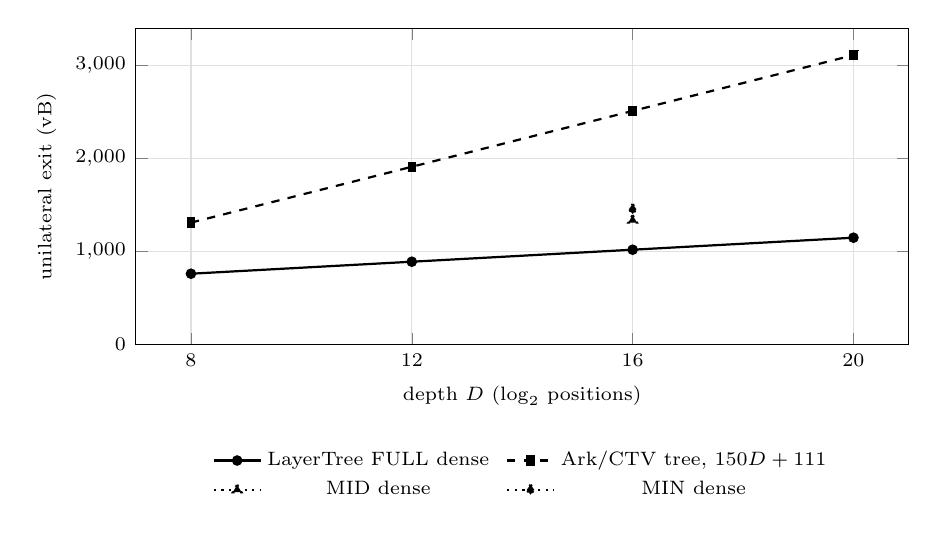
\begin{tikzpicture}
\begin{axis}[
  width=0.94\linewidth, height=5.6cm,
  xlabel={depth $D$ ($\log_2$ positions)}, ylabel={unilateral exit (vB)},
  xmin=7, xmax=21, ymin=0, ymax=3400,
  xtick={8,12,16,20}, grid=major, grid style={black!12},
  legend style={at={(0.5,-0.3)}, anchor=north, legend columns=2, font=\scriptsize, draw=none, fill=none, /tikz/every even column/.append style={column sep=4pt}},
  tick label style={font=\scriptsize}, label style={font=\scriptsize}
]
\addplot[thick, mark=*, mark size=1.5pt] coordinates {(8,762) (12,891) (16,1020) (20,1149)};
\addlegendentry{LayerTree FULL dense}
\addplot[thick, dashed, mark=square*, mark size=1.5pt] coordinates {(8,1311) (12,1911) (16,2511) (20,3111)};
\addlegendentry{Ark/CTV tree, $150D+111$}
\addplot[thick, dotted, mark=triangle*, mark size=1.8pt] coordinates {(16,1338)};
\addlegendentry{MID dense}
\addplot[thick, dotted, mark=diamond*, mark size=1.8pt] coordinates {(16,1456)};
\addlegendentry{MIN dense}
\end{axis}
\end{tikzpicture}
\end{minipage}\hfill
\begin{minipage}[b]{0.38\linewidth}\centering
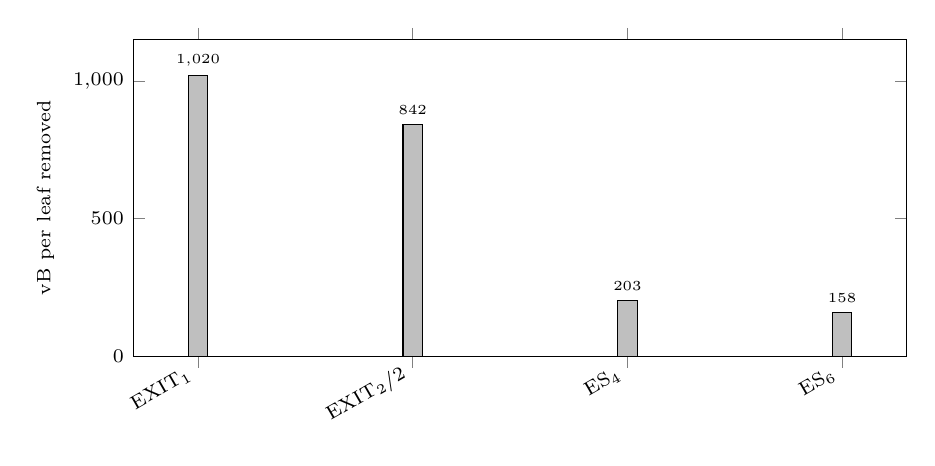
\begin{tikzpicture}
\begin{axis}[
  width=0.94\linewidth, height=5.6cm,
  ybar, bar width=7pt,
  symbolic x coords={EXIT$_1$, EXIT$_2$/2, ES$_4$, ES$_6$},
  xtick=data, ylabel={vB per leaf removed}, ymin=0, ymax=1150,
  nodes near coords, nodes near coords style={font=\tiny},
  tick label style={font=\scriptsize}, label style={font=\scriptsize},
  x tick label style={rotate=30, anchor=east}
]
\addplot[fill=black!25] coordinates {(EXIT$_1$,1020) (EXIT$_2$/2,842) (ES$_4$,203) (ES$_6$,158)};
\end{axis}
\end{tikzpicture}
\vspace{7mm}
\end{minipage}
\caption{Left: unilateral exit cost against tree depth, measured for LayerTree and modelled for a transaction tree. Right: per-leaf cost of removal at $D=16$: a single exit, the average of a two-exit batch, and cohort sweeps \tr{EVICT\_SUBTREE}$_4$ (13 leaves) and $_6$ (51 leaves).}
\label{fig:plot}
\end{figure}

\paragraph{Batching and cohorts.} A second exit in the same transaction
costs $665\vB$ marginally against $1{,}020\vB$ alone, since the prologue,
key recomputation and skeleton are shared. Grafting is the decisive
difference between the profiles for onboarding: a dense \tr{JOIN}$_h$
adds any number of members for a constant $\approx 2{,}000\WU$, while
sparse joins cost $\approx 5{,}000\WU$ per leaf however they are batched.
Cohort sweeps do for removal what grafting does for addition:
\tr{EVICT\_SUBTREE}$_4$ removes 13 leaves at $203\vB$ each and
\tr{EVICT\_SUBTREE}$_6$ removes 51 at $158\vB$ each, a 5 to 6.5$\times$
reduction over individual evictions that improves with cohort size
because the subtree's interior is hashed once. Operators therefore graft
members who share a lease expiry into one aligned subtree, and both add
and remove the cohort in one constant-shape transaction each.

\paragraph{Fees.} At $10\sat/\mathrm{vB}$ a $D=16$ exit costs
$10{,}200\sat$, so a balance of $1{,}020{,}000\sat$ exits for a 1\% fee
and $102{,}000\sat$ for 10\%; at $50\sat/\mathrm{vB}$ the figures are
five times higher. Cohort sweeps keep small leaves evictable at high
rates: $158\vB$ per leaf is $7{,}900\sat$ at $50\sat/\mathrm{vB}$.
Dust is never the binding constraint for $D \ge 8$; the fee is. Varops
usage is 6 to 8\% of the BIP-440 budget in the dense profile and 8 to 25\%
in the sparse profile, dominated by the EC operations and the signature at
small depths and by hashing at large ones.

\paragraph{Channel leaves.} A force-close of a channel leaf at $D = 16$
is the exit ($1{,}020\vB$), an update transaction ($153\vB$) and its
anchor child, and after the delay a settlement ($204\vB$ plus $43\vB$ per
HTLC) and its child: about $1{,}680\vB$ in total, of which the channel
machinery is about $660\vB$. It is roughly 13$\times$ a Lightning force
close, and the difference is exactly the price of never having had the
funding output on-chain; cooperative closes, splices and lease renewals
cost one tree transition or nothing.

\section{Related Work}\label{sec:related}

Channel factories~\cite{factories} share one output among $N$ channels
but require all $N$ to sign every factory-level change and publish a
transaction tree to exit. Ark~\cite{ark} batches users into rounds whose
virtual outputs are leaves of a pre-signed or CTV-committed tree; exit
unrolls the branch, the round expires, and users must refresh. Timeout
trees~\cite{timeouttrees} and MATT-style covenant trees~\cite{matt,bip443}
replace signatures by templates but keep the transaction tree and its
$O(\log N)$ exit. Statechains~\cite{statechains} transfer a whole UTXO
off-chain but do not divide it. LayerTree differs from all of these in
that the tree is data rather than transactions: exit is $O(1)$
transactions and $O(D)$ bytes, the interior needs no pre-signing, the
operator can evict, and the output never expires.
Table~\ref{tab:compare} summarises.

\begin{table}[t]
\centering\small
\caption{Comparison with shared-output constructions.}
\label{tab:compare}
\setlength{\tabcolsep}{3pt}\scriptsize
\begin{tabular}{@{}lllll@{}}
\toprule
 & LayerTree & Ark & Timeout tree & CTV/CCV tree \\
\midrule
Unilateral exit & 1 tx, $O(D)$ B & $O(\log N)$ txs & $O(\log N)$ txs & $O(\log N)$ txs \\
Evict one leaf & 1 tx after lease & tree expires & tree expires & no \\
Interactive signing & none & round members & all & none \\
Shared output expiry & none & per round & per tree & per design \\
Batch add & 1 tx, any subtree & per round & per tree & per tree \\
Off-chain payments & channel leaves, vouchers & out-of-round & channels & varies \\
Opcodes & GSR, \op{TX}, CSFS, EC & none / CTV & CTV & CTV / CCV \\
\bottomrule
\end{tabular}
\end{table}

The Merkle-sum sparse Merkle tree is taken from Taproot
Assets~\cite{mssmt}, where it commits to asset balances; here it is
truncated in depth and its verification moved into script. The
data-tweaked internal key follows the pattern of
\op{CHECKCONTRACTVERIFY}~\cite{bip443}, realised from EC opcodes. The
channel state machine is eltoo~\cite{eltoo}; its \texttt{ANYPREVOUT}
requirement~\cite{bip118} is met here by collated introspection and
\op{CHECKSIGFROMSTACK} rather than a new sighash flag, and unlike
CTV-based LN-Symmetry no script data need be retained to respond to a
published state. The constructive introspection of \S\ref{sec:min} is in
the tradition of covenant tricks that recover transaction data from a
signature check; we are not aware of a prior use of a generator-key
signature with $s = e + 1$ to make the script's reconstruction binding.

\section{Discussion and Limitations}\label{sec:discussion}

\paragraph{What the covenant does and does not guarantee.} It guarantees
conservation and the payability of every leaf under a grounded node. It
does not guarantee that the operator will add you (a member who is never
added has lost nothing), nor that the operator's grafted nodes have
preimages (a member who funds a join without verifying its path inside the
subtree has trusted the operator). The specification makes the check
mandatory, and the Lean development shows it is load-bearing.

\paragraph{Exit serialisation.} Every transition spends the same UTXO.
Cooperative batching makes this a non-issue for a responsive operator; an
uncooperative mass exit is bounded by mempool descendant policy to about
25 leaves per block. Trees should be sized by this throughput, not by
depth, and channel-hosting trees by it against HTLC deadlines. This is a
property of the single-UTXO design and cannot be engineered away within
it; sharding is the answer.

\paragraph{Operator power.} The operator cannot steal, freeze provable
leaves, or block exits. It can evict any leaf after its lease and, in a
cohort tree, many at once for about $160\vB$ each, which makes griefing
cheap for it. Members who want a hard guarantee buy it with a future lease
height and, for channel leaves, give up routing until it passes.

\paragraph{Opcode dependence.} The design is hostage to proposals. Its
strongest dependency is on a tapleaf version with restored string opcodes
or, failing that, \op{CAT}; \op{TX} in \texttt{0xC0} is assumed for the
MID tier and its selector values are drafts; the EC opcodes' operand order
and cost are drafts. Every selector and opcode number is a named constant
in the implementation.

\paragraph{Future work.} The off-chain protocol (joins, cohorts, channel
leaves under an adversarial scheduler) is a different kind of object from
the covenant and wants a model checker; we have a design for a P
model~\cite{plang}. A verified interpreter for the tapscript subset would
close the gap between the rules the Lean model proves and the bytecode the
tests execute. Hash-locked vouchers give atomic swaps between the credit
instrument and channel HTLCs inside one tree. Aggregate node keys would
allow Ark-style cooperative subtree replacement in one signature, at the
cost of the interactive round the design set out to avoid.

\section{Conclusion}

A shared Bitcoin output whose tree lives off-chain as data rather than
transactions gives every member a one-transaction exit of about a
kilobyte, gives the operator eviction and cohort sweeps, needs no
pre-signing and never expires. The construction uses only opcodes already
on the table, and the minimum it truly needs is \op{CAT} and a point
tweak. Its guarantees are theorems in the idealised hash model, checked
mechanically, and its costs are measured by execution. The price is that
all activity funnels through one UTXO, which bounds how fast a tree can be
dissolved against its will; we regard that as the honest trade-off of the
approach and the parameter operators must design around.

\bibliographystyle{splncs04}
\bibliography{refs}

\appendix
% Appendix: the Lean formalisation. Input from main.tex after \appendix.
\section{The Lean Formalisation}\label{app:lean}

This appendix describes the mechanised model behind \S\ref{sec:security}
in enough detail that a reader can judge what has been proved, under
what assumptions, and what has not. The development is about 1{,}300
lines of Lean~4~\cite{lean4} in seven modules and depends on nothing but the
core library: no Mathlib, no external tactics. It builds in seconds and
prints an axiom audit for every headline theorem; each depends only on
\lean{propext}, \lean{Quot.sound} and, in one case, \lean{Classical.choice},
and none on \lean{sorryAx}. The code is in the artefact~\cite{layertreerepo}.

\subsection{Design of the Model}

The model states the \emph{rules} of \S\ref{sec:transitions} as
relations over the objects the scripts manipulate: nodes, paths, amounts.
It does not model tapscript bytecode, signatures, keys or lock times.
Authorisation is carried as an opaque proposition, and the input and
output amounts the scripts read with \op{TX} are parameters. Three
choices keep the proofs short.

\paragraph{Depth as a type index.} A tree of depth $d$ is
\lean{Tree d}, a perfect binary tree whose tips are \lean{Option Leaf}.
Positions are \lean{Pos d h}, paths from depth $d$ down to a subtree of
height $h$, so that \lean{Pos d 0} addresses a leaf and \lean{Pos d h}
addresses the slot a \tr{JOIN}$_h$ fills. Indexing by both endpoints
avoids all arithmetic on depths: the recursions on \lean{getSub},
\lean{setSub} and \lean{pathSub} pattern-match on the position and the
tree simultaneously, and the one impossible case (a \lean{cons} step below
height~$0$) is dismissed by \lean{Pos.height\_le}.

\begin{lstlisting}
inductive Tree : Nat → Type
  | tip : Option Leaf → Tree 0
  | bin {d : Nat} : Tree d → Tree d → Tree (d + 1)

inductive Pos : Nat → Nat → Type
  | nil {h : Nat} : Pos h h
  | cons {d h : Nat} : Bool → Pos d h → Pos (d + 1) h

def parent (a b : Node H) : Node H :=
  ⟨M.hNode a.hash a.sum b.hash b.sum, a.sum + b.sum⟩

def combine (n : Node H) (x : Bool × Node H) : Node H :=
  if x.1 then parent x.2 n else parent n x.2

def fold (n : Node H) : List (Bool × Node H) → Node H
  | [] => n
  | x :: rest => combine (fold n rest) x
\end{lstlisting}

\paragraph{Root-first paths.} The model orders a sibling path from the
root down, so \lean{fold} is a structural recursion on the list and the
soundness proof is a plain induction. The witness of \S\ref{sec:scripts}
supplies the same pairs leaf-first, because the script consumes the
deepest level first; nothing in the theorems depends on the order.

\paragraph{Hashes as parameters.} Everything is parametric in a class
\lean{HashModel} whose fields are the two hash functions, the zero digest,
and the assumptions the argument uses:

\begin{lstlisting}
class HashModel (Leaf : Type) (H : outParam Type) where
  hLeaf : Leaf → H
  hNode : H → Nat → H → Nat → H
  empty0 : H
  hLeaf_inj : ∀ {l₁ l₂}, hLeaf l₁ = hLeaf l₂ → l₁ = l₂
  hNode_inj : ∀ {a₁ b₁ a₂ b₂ sa₁ sb₁ sa₂ sb₂},
    hNode a₁ sa₁ b₁ sb₁ = hNode a₂ sa₂ b₂ sb₂ →
      a₁ = a₂ ∧ sa₁ = sa₂ ∧ b₁ = b₂ ∧ sb₁ = sb₂
  hNode_ne_hLeaf : ∀ a sa b sb l, hNode a sa b sb ≠ hLeaf l
  hNode_ne_empty : ∀ a sa b sb, hNode a sa b sb ≠ empty0
  hLeaf_ne_empty : ∀ l, hLeaf l ≠ empty0
\end{lstlisting}

Injectivity is collision resistance idealised; the three inequalities are
the tag separation that distinct BIP-340 tags provide. The encodings
module discharges the serialisation half of each injectivity field
(Lemma~\ref{lem:enc}): given SHA-256 collision resistance,
\lean{serializeLeaf\_inj} and \lean{serializeNode\_inj} are what remains.
Nothing quantifies the adversary's advantage; a proof under injectivity
transfers to any adversary that cannot exhibit a collision.

\subsection{Theorem Statements}

The statements below are verbatim from the development. \lean{t.root} is
the root node of a tree, \lean{t.getSub p} the subtree at position
\lean{p}, \lean{t.setSub p u} the tree with that subtree replaced by
\lean{u}, \lean{t.pathSub p} the honest sibling path, and \lean{t.get},
\lean{t.set}, \lean{t.path} their leaf-level specialisations.

\begin{lstlisting}
theorem fold_pathSub (t : Tree d) (p : Pos d h) :
    fold (t.getSub p).root (t.pathSub p) = t.root

theorem fold_setSub (t : Tree d) (p : Pos d h) (s : Tree h) :
    fold s.root (t.pathSub p) = (t.setSub p s).root

theorem root_inj (t₁ t₂ : Tree d) : t₁.root = t₂.root → t₁ = t₂

theorem fold_sound (t : Tree d) (m : Node H) (π : List (Bool × Node H)) :
    fold m π = t.root →
    ∃ (h : Nat) (p : Pos d h), m = (t.getSub p).root ∧ π = t.pathSub p
\end{lstlisting}

\lean{fold\_sound} is Theorem~\ref{thm:binding}. Its proof is the only
place the hash axioms are used: a non-empty path claims an internal node,
so the tree is not a tip by tag separation, and injectivity of
\lean{hNode} equates both children's hashes and sums with the claimed
ones. Note that the conclusion equates \emph{nodes}, so the sum the
prover presented is the true sum of the subtree.

A \lean{Step} is a path, a height, an old node and a new node; it is
valid for roots $r, r'$ when the old node folds to $r$ and the new node to
$r'$, and well formed for depth $d$ when the path has $d - h$ entries.
\lean{Steps} chains steps, each against the root the previous one produced.

\begin{lstlisting}
theorem Step.sound (t : Tree d) (s : Step H) (r' : Node H)
    (hwf : s.WF d) (hv : s.valid t.root r') :
    ∃ p : Pos d s.height, s.old = (t.getSub p).root ∧
      ∀ (u : Tree s.height), u.root = s.new → r' = (t.setSub p u).root

theorem Steps.sum (h : Steps r ss r') :
    r'.sum + oldSum ss = r.sum + newSum ss

theorem Steps.sound (t : Tree d) (h : Steps t.root ss r')
    (hwf : ∀ s ∈ ss, s.WF d) (hg : ∀ s ∈ ss, s.Grounded) :
    ∃ t' : Tree d, t'.root = r'
\end{lstlisting}

\lean{Steps.sum} is Theorem~\ref{thm:cons} and needs no hash assumption.
\lean{Steps.sound} is Theorem~\ref{thm:ground}; \lean{s.Grounded} says
the new node is the root of some tree of the step's height, which
leaf-level steps satisfy by construction (\lean{grounded\_of\_leaf}) and
which a \tr{JOIN} graft must be given.

The transitions are structures bundling the steps with the output rule
and an opaque authorisation. Their theorems:

\begin{lstlisting}
theorem payable (t : Tree d) (p : Pos d 0) (l : Leaf) (hl : t.get p = some l) :
    (leafStep (t.path p) (some l) none).valid t.root (t.set p none).root ∧
    (t.set p none).root.sum + l.amount = t.root.sum ∧
    ∀ q, q ≠ p → (t.set p none).get q = t.get q

theorem ExitK.no_inflation (h : ExitK exact r blocks r' out0) :
    out0 + payoutSum blocks ≤ r.sum

theorem ExitK.exact_conservation (h : ExitK true r blocks r' out0) :
    out0 + payoutSum blocks = r.sum

theorem join_sound (t : Tree d) (hwf : path.length + h = d)
    (hj : Join auth h t.root path new r' out0) :
    ∃ p : Pos d h, t.getSub p = Tree.empty h ∧
      out0 = t.root.sum + new.sum ∧
      ∀ u : Tree h, u.root = new → r' = (t.setSub p u).root

theorem claim_sound (t : Tree d) (hwf₁ : srcPath.length = d)
    (hwf₂ : claimPath.length = d)
    (hc : Claim auth t.root srcPath claimPath src claim r' out0) :
    out0 = t.root.sum ∧
    ∃ (p₁ p₂ : Pos d 0), t.get p₁ = some src ∧
      (t.set p₁ (claimedSource src claim.amount)).get p₂ = none ∧
      r' = ((t.set p₁ (claimedSource src claim.amount))
              .set p₂ (some claim)).root
\end{lstlisting}

\lean{payable} is Theorem~\ref{thm:pay}. \lean{join\_sound} uses
\lean{root\_inj} (via \lean{eq\_empty\_of\_root}): since \tr{JOIN}$_h$
hard-codes $\Emp_h$ as the old node, the slot it fills is provably the
empty tree, and the theorem gives the successor root for every tree whose
root is the grafted node. \lean{claim\_sound} exposes the drained-source
case: the claim position must be empty in the tree \emph{after} the source
step, which is why a source reduced to zero may host the claim.

\subsection{Assumption Ledger}

Every hypothesis outside Lean's logic, what it stands for in the
deployment, and which theorems consume it.

\begin{center}\scriptsize
\begin{tabular}{@{}p{3.6cm}p{4.2cm}p{3.6cm}@{}}
\toprule
hypothesis & stands for & used by \\
\midrule
\lean{hLeaf\_inj} & SHA-256 collision resistance + \lean{serializeLeaf\_inj} & \lean{leafNode\_inj}, \lean{root\_inj} \\
\lean{hNode\_inj} & SHA-256 collision resistance + \lean{serializeNode\_inj} & \lean{root\_inj}, \lean{fold\_sound} \\
\lean{hNode\_ne\_hLeaf}, \lean{hNode\_ne\_empty}, \lean{hLeaf\_ne\_empty} & distinct tags (random-oracle heuristic) & \lean{leafNode\_inj}, \lean{fold\_sound} \\
\lean{treeSpk\_inj} & DL on secp256k1 + CR of $\Hstate$, TapTweak & \lean{witness\_root\_binds} \\
real-tree invariant & creation check + grounded grafts (off-chain) & every theorem stated for a \lean{Tree} \\
\midrule
(none) & & \lean{Steps.sum}, \lean{ExitK.no\_inflation}, encodings \\
\bottomrule
\end{tabular}
\end{center}

The conservation results use no hypothesis at all, which is the formal
content of ``the covenant conserves sums whatever it is shown''. The
collision-resistance assumption on the TapSighash and challenge hashes
that the MIN tier's constructive introspection adds (\S\ref{sec:min}) is
outside the model, since the model does not include signature checking.

\subsection{Modules and Effort}

\begin{center}\scriptsize
\begin{tabular}{@{}lrp{7.5cm}@{}}
\toprule
module & lines & contents \\
\midrule
\lean{Hash.lean} & 59 & the \lean{HashModel} class \\
\lean{Leaf.lean} & 96 & \lean{Leaf}, \lean{Leaf.WF}, \lean{Node}, \lean{leafNode}, \lean{leafNode\_inj} \\
\lean{Tree.lean} & 335 & trees, positions, paths, \lean{fold}, all tree theorems \\
\lean{Transitions.lean} & 458 & \lean{Step}, \lean{Steps}, the transitions and their theorems \\
\lean{Binding.lean} & 60 & \lean{BindingModel} and the two binding theorems \\
\lean{Encoding.lean} & 238 & encodings, serialisation injectivity, \lean{SEQ\_FINAL} \\
\lean{Axioms.lean} & 32 & the axiom audit \\
\bottomrule
\end{tabular}
\end{center}

The only proofs that took real effort were \lean{fold\_sound}, where the
two-index positions and the domain-separation case for a tip had to be
found, and \lean{Steps.sound}, where the height of the grounding tree
must be reconciled with the height the soundness lemma returns, which is
why \lean{Step} carries its height explicitly. A verified interpreter for
the tapscript subset would need a model of the stack machine, of
BIP-441 numerics, of \op{TX}'s serialisations and of the BIP-341 message,
and a proof that each generated script's execution relation equals the
corresponding \lean{Step} relation; we estimate it at several thousand
lines and regard it as the natural sequel.

\subsection{Binding to the Output}

\lean{Binding.lean} records the one cryptographic step outside the hash
model. A structure \lean{BindingModel} carries an abstract
\lean{treeSpk : H → TapRoot → Spk} with the hypothesis that it is
injective in both arguments, and two one-line theorems conclude that a
witness $(r', m')$ passing the scriptPubKey check equals the committed
$(r, m)$, and that the successor output commits to the computed root under
the same $m$. In the deployment the map is
$(r, m) \mapsto x\bigl(P_r + H_{\mathsf{TapTweak}}(x(P_r) \,\|\, m)\cdot G\bigr)$
with $P_r = \mathsf{lift\_x}(x(\NUMS + \Hstate(r) G))$, and the two
x-projections identify a point with its negation. A collision
$(r, m) \ne (r', m')$ yields one of: $x(P_r) = x(P_{r'})$ with $r \ne r'$,
which is a collision in $\Hstate$ or the relation
$\NUMS + tG = -(\NUMS + t'G)$, solvable for the discrete logarithm of
$\NUMS$; $x(P_r) = x(P_{r'})$ with $m \ne m'$, a collision in
$H_{\mathsf{TapTweak}}$; or distinct internal keys with $Q = \pm Q'$,
again a linear relation in $\NUMS$ and $G$ solvable for the discrete
logarithm of $\NUMS$. Making the hypothesis explicit is the point: it is
what a future script change must not break.

\subsection{Encodings}

\lean{Encoding.lean} proves the byte-level facts the design leans on, over
natural-number bytes so that every proof stays within linear arithmetic:
fixed-width little-endian encodings are injective on their range;
\lean{minimalLE (n + 2\^{}(8k)) = leBytes k n ++ [1]} for $n < 2^{8k}$,
which with $k = 8$ is $\encs$ and justifies producing it with one
addition; the 116-byte leaf and the 82-byte node preimage are injective;
and the \lean{SEQ\_FINAL} facts of Lemma~\ref{lem:enc}, computed by
\lean{decide} on a bounded-recursion model of \texttt{CScriptNum}.

\subsection{What Is Not Proved}

The tapscript bytecode is outside the model. That the scripts of
\S\ref{sec:scripts} implement the relations above is established by
execution: every script of every tier runs in the simulator against a
reference tree with positive and negative cases, and the Go generators are
compared byte for byte with the Python output. A verified interpreter for
the tapscript subset (BIP-441 numerics, \op{TX}, \op{CHECKSIGFROMSTACK})
would close this gap and is a project of a different size. Signatures,
lock times and the transaction structure beyond amounts are
authorisation-side facts and are deliberately opaque. Concurrency,
mempool policy, reorganisations and the off-chain protocol are not
theorems about hash trees and belong to a model checker; a design for a
P~\cite{plang} model is in the artefact.


\end{document}
